\documentclass[11pt]{article}
\usepackage[margin=1in]{geometry}
\usepackage{amsmath,amssymb}
\usepackage{graphicx}
\usepackage{tikz}
\usetikzlibrary{calc}
\usepackage{pgfplots}
\pgfplotsset{compat=1.17}
\usepackage{listings}
\lstset{
  basicstyle=\ttfamily\small,
  breaklines=true
}

\title{Comprehensive Review: The AdaBoost Algorithm}
\author{Master's Level Data Science}
\date{}

\begin{document}
\maketitle
\tableofcontents
\bigskip

\section{Introduction}
This review synthesizes the lecture slides (\texttt{ensemble-2.pdf}) and audio transcript (\texttt{AdaBoostAlgorithm.txt}) on the AdaBoost algorithm. We cover the motivation for boosting weak learners, the AdaBoost procedure, theoretical guarantees, a worked example, and practical considerations.

\section{Motivation: Weak Learners and Boosting}
A \emph{weak learner} is an algorithm that, on any distribution over examples $(x_i,y_i)$ with labels $y_i\in\{-1,+1\}$, returns a hypothesis $h$ with error
\[
  \Pr\bigl(h(X)\neq Y\bigr)\;\le\;\tfrac12 - \epsilon,
\]
for some $\epsilon>0$. Boosting is a method to convert such weak learners into a \emph{strong learner} with arbitrarily low training error by combining multiple hypotheses in a weighted vote.

\section{The AdaBoost Algorithm}
Given a training set $\{(x_i,y_i)\}_{i=1}^n$, initialize weights
\[
  D_1(i) \;=\;\frac1n,\quad i=1,2,\dots,n.
\]
For rounds $t=1,\dots,T$:
\begin{enumerate}
  \item Train weak learner on weighted sample $D_t$ to obtain $h_t:X\to\{-1,+1\}$.
  \item Compute weighted error
  \[
    \varepsilon_t 
    = \sum_{i=1}^n D_t(i)\,\mathbf{1}[h_t(x_i)\neq y_i].
  \]
  \item Compute classifier weight
  \[
    \alpha_t
    = \frac12\ln\!\Bigl(\frac{1-\varepsilon_t}{\varepsilon_t}\Bigr).
  \]
  \item Update weights for all $i$:
  \[
    D_{t+1}(i)
    = \frac{D_t(i)\,\exp\bigl(-\alpha_t\,y_i\,h_t(x_i)\bigr)}
           {\sum_{j=1}^n D_t(j)\,\exp\bigl(-\alpha_t\,y_j\,h_t(x_j)\bigr)}.
  \]
\end{enumerate}
The final strong classifier is
\[
  H(x) \;=\;sign\Bigl(\sum_{t=1}^T \alpha_t\,h_t(x)\Bigr).
\]

\section{Theoretical Guarantee}
If each weak hypothesis has edge $\gamma_t = \tfrac12 - \varepsilon_t>0$, then the training error of $H$ satisfies
\[
  \frac1n\sum_{i=1}^n \mathbf{1}[H(x_i)\neq y_i]
  \;\le\;\exp\!\Bigl(-2\sum_{t=1}^T \gamma_t^2\Bigr)
  \;\le\;\exp\!\Bigl(-2T\gamma^2\Bigr),
\]
where $\gamma = \min_t\gamma_t$. Thus training error decays exponentially in $T$.

\section{Worked Example (Freund--Schapire)}
We illustrate on a toy set with decision stumps as weak learners.

\subsection{Example Data and Results}
\begin{center}
\begin{tabular}{c|ccc}
 & $D_1$ & $D_2$ & $D_3$ \\
\hline
$h_1$ & $\varepsilon_1=0.40,\;\alpha_1=0.42$ & & \\
$h_2$ & & $\varepsilon_2=0.42,\;\alpha_2=0.37$ & \\
$h_3$ & & & $\varepsilon_3=0.30,\;\alpha_3=0.42$ \\
\end{tabular}
\end{center}
After three rounds, the combined classifier is
\[
  H(x) = sign\bigl(0.42\,h_1(x) \;+\; 0.37\,h_2(x)\;+\;0.42\,h_3(x)\bigr),
\]
which can perfectly separate the training set.

\section{Geometric Illustration}
\begin{figure}[h]
\centering
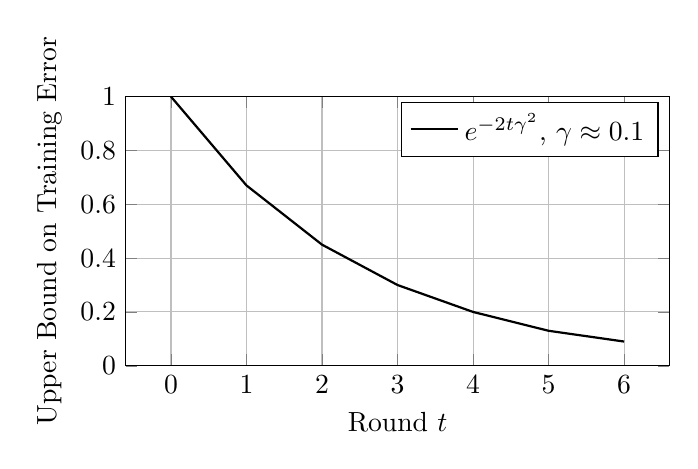
\begin{tikzpicture}
  \begin{axis}[
    width=0.7\textwidth,
    height=5cm,
    xlabel={Round $t$},
    ylabel={Upper Bound on Training Error},
    ymin=0, ymax=1,
    grid=both
  ]
    \addplot[thick] table[row sep=\\] {
t   bound\\
0   1.00\\
1   0.67\\
2   0.45\\
3   0.30\\
4   0.20\\
5   0.13\\
6   0.09\\
};
    \addlegendentry{$e^{-2t\gamma^2}$, $\gamma\approx0.1$}
  \end{axis}
\end{tikzpicture}
\caption{Exponential decay of the training error bound with rounds of boosting.}
\end{figure}

\section{Algorithm Summary}
\begin{enumerate}
  \item Initialize uniform weights on examples.
  \item For each round:
    \begin{enumerate}
      \item Train weak learner on weighted data.
      \item Compute error and hypothesis weight.
      \item Reweight examples to emphasize mistakes.
    \end{enumerate}
  \item Output sign of weighted vote of hypotheses.
\end{enumerate}

\section{Practical Considerations}
\begin{itemize}
  \item \textbf{Choice of Weak Learner}: Decision stumps are common; deeper trees can be used.
  \item \textbf{Overfitting}: Monitor validation error; limiting $T$ or adding shrinkage can help.
  \item \textbf{Computational Cost}: Each round requires retraining on weighted data.
  \item \textbf{Extensions}: Gradient boosting generalizes to arbitrary losses.
\end{itemize}

\section{Future Directions}
\begin{itemize}
  \item \textbf{Gradient Boosting Machines}: Use differentiable loss and regression trees.
  \item \textbf{Regularization Schemes}: Subsample data (\emph{bagging}), shrinkage.
  \item \textbf{Multi-class Boosting}: SAMME and variants for multiple labels.
  \item \textbf{Applications}: Ranking, regression, anomaly detection.
\end{itemize}

\end{document}
